\documentclass[conference]{IEEEtran}
\IEEEoverridecommandlockouts
% The preceding line is only needed to identify funding in the first footnote. If that is unneeded, please comment it out.
\usepackage{cite}
\usepackage{amsmath,amssymb,amsfonts}
\usepackage{algorithmic}
\usepackage{float}
\usepackage{graphicx}
\usepackage{hyperref}
\usepackage{textcomp}
\def\BibTeX{{\rm B\kern-.05em{\sc i\kern-.025em b}\kern-.08em
    T\kern-.1667em\lower.7ex\hbox{E}\kern-.125emX}}
\linespread{2.0}
\begin{document}

\title{K-Means Genetic Programming\\
\thanks{*Josh earned his Bachelor of Science in Computer Science in May 2016.  He is a former member of the Natural Computation Laboratory at the Missouri University of Science and Technology.  Josh hopes to graduate with a Master of Science in Computer Science in May 2018.}
}

\author{\IEEEauthorblockN{Joshua M. Tuggle*}
\IEEEauthorblockA{May 3, 2018 \\
CS 6405 - Clustering Algorithms}}

\maketitle

\onecolumn
\tableofcontents
\clearpage


\section{Executive Summary}
The purpose of this paper is to create a faster running k-means clustering algorithm.  This is achieved by providing a training dataset for the algorithm to train.  The training process involves using Genetic Programming to evolve parse trees.  These transform all the features that a point has into a single feature.  The hope is that using the evolved parse tree on a new dataset, it can reduce the features of the points.  As a consequence of this, the time it takes to calculate the distance between a point and a cluster is reduced.  This project is not only here to see if such a speed increase is possible, but to also investigate if there is a difference in solution purity between the evolved k-means method and base k-means.

\clearpage

\section{Introduction}
\subsection{Clustering}
The ability to classify data is an important part of data science.  The more tools that we have at our disposal, the better prepared we are for dealing with the complexities the world throws at us.  When dealing with algorithms, we typically want our algorithms as fast and accurate as possible.

\subsection{K-Means Clustering}
The k-means clustering method is a simple and powerful way of clustering data.  The idea behind k-means clustering is that given a dataset and a value K, the algorithm will partion the dataset into k different groups.  The algorithm will initially pick K random points from the dataset and will set the center of each of the clusters to those randomly chosen points.  Next, k-means will iterate over every point and for each point it will determine to which cluster it is closest and will assign the point to it.  The way k-means computes distance between two points is Euclidean distance\cite{Xu2005}.  The formula for Euclidean Distance can be seen in Figure 1.  K-means will then go though every cluster and calculate a new center point for the cluster based on the average of the points assigned to it.  The algorithm will then go back to the step where it iterates over all the points and finds the closest cluster.  This process repeats until none of the points are reassigned to a cluster.  K-means will then return the cluster assignment to where each point belongs.

\begin{figure}[htbp]
\begin{center}
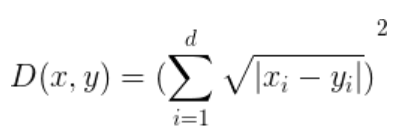
\includegraphics[width=0.4\columnwidth]{EuclideanDistance.png}
\caption{Formula for Euclidean distance.}
\end{center}
\label{fig}
\end{figure}

On the surface, k-means clustering it has been shown to have a time complexity of O(NKdT) \cite{XuRui2008}.  This is where N is the number of points in the dataset, K is the number of clusters desired in k-means, d is the dmensionality of the data (number of features), and T is the number of iterations for termination of k-means.  The speed of k-means could be hurt quite significantly if there were a large number of features.  If the number of features were transformed into 1, then that would be d = 1.  Given that the other factors stay constant, the runtime of k-means would become O(NKT).  This O(NKT) k-means method could theoretically be as fast or faster than the O(NKdT) k-means method.  The thing to do would be to find a way to transform all the features into a new feature.

\subsection{Evolutionary Algorithms/Genetic Programming}
Evolution Algorithms (EAs) and Genetic Programming (GPs) are tools that can solve optimization and machine learning respectively\cite{EibenAE2007}.  GPs take the form of trees and can be used as parse trees.

\begin{figure}[H]
\begin{center}
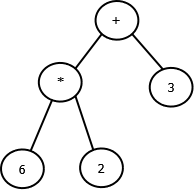
\includegraphics[width=0.4\columnwidth]{ParseTreeExample.png}
\caption{An example GP/parse tree.}
\end{center}
\label{fig}
\end{figure}

The above example of a parse tree can really be represented as the (6 * 2) + 3.  This expression is equal to 15.  The are numbers in the tree are called terminals, while the math operators in the tree are called non-terminals/functions.  Imagine that instead of just having random numbers in the terminals spot in the parse tree, there were instead features from a dataset.  By taking  random features from a point, a parse tree would produce a single value.  That value would become the single feature representing that point.  Having that single feature could lead to a speed up in k-means.  The power of EAs/GPs is that they create new trees in the problem space and can allow strong performing parse trees to rise to the top\cite{EibenAE2007}.

\clearpage

\section{Project Specifications}
The purpose of this project is that given a dataset, the project framework, KMeansGP, will evolve a parse tree that can reduce the number of features of a point to one.  Whenever a new dataset of a problem class that already has an evolved parse tree appears, then the features of the points can each be reduced to a single feature.  This storage of prepared heuristics to use at a later has been in \cite{Illetskova2017}.  K-means clustering is then performed on these single feature points and will ideally be faster than if you never reduced the features of the points.  Ideally, not only would the reduced feature points solution be faster, but the solution would not lose little to no accuracy.  This project is a testbed for seeing if combining Genetic Programming with k-means clustering can make these goals possible.
\clearpage

\section{Detailed Design}
\subsection{Framework}
This project is a testbed for testing if k-means clustering and Genetic Programming can be put together to produce faster run times of k-means clustering.  Below is the framework behind the project.

\begin{figure}[H]
\begin{center}
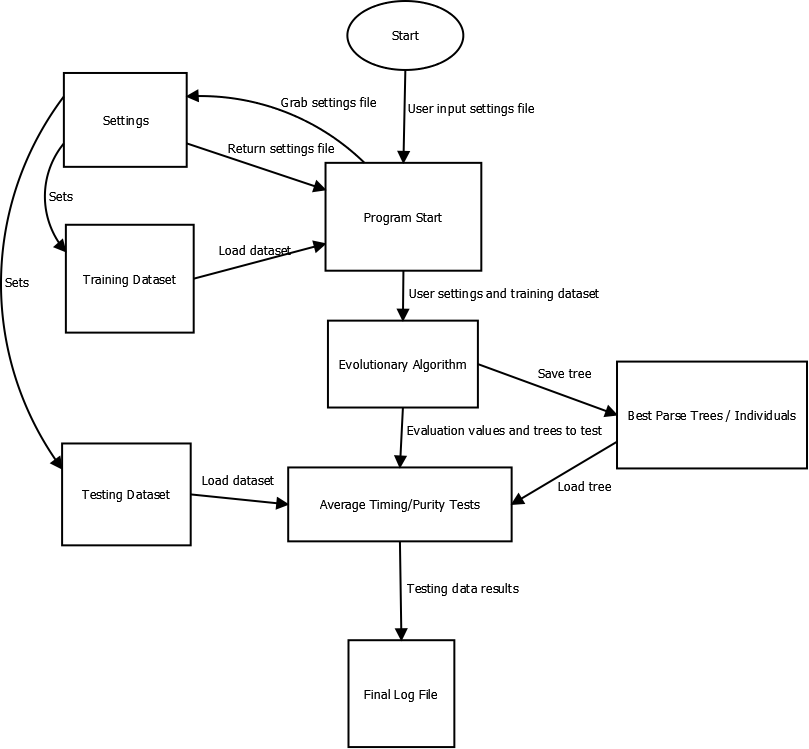
\includegraphics[width=0.8\columnwidth]{Architecture.png}
\caption{KMeansGP Framework.}
\end{center}
\label{fig}
\end{figure}

The KMeansGP framework was written in C++.  The first reason that C++ was chosen is because it is one of the fastest langauges out there\cite{Aruboa2014}.  As a consequence of C++ being a fast language, this would allow fitness evaluations for the EA to be done at a much faster time.  The other reason is that the author wanted to practice writing some of the basic EA features in C++ for fun.

As designed, the framework itself is fairly generic.  The settings and tasks for the programming are really made in the settings file.  This allows the user to tell the program where the training and testing datasets are located.  The settings file also contains some customizable parameters for the EA run.  As the author needed an easy way to access the data from running the code, a log file is generated near the end of the code run.
\subsection{Representation of a Tree}
The author had to figure out a way to implement parse trees in C++ without using any special external tree libraries.  After some research, parse trees using binary heaps\cite{HodaNima} was implemented.  The thing is about binary heaps is that they can implemented using C++ vectors, which are basically a resizable arrays.  One of features that needed to be in this program was the ability to save and load parse trees from a file.  The size of the vector that held the parse tree could be stored in the file.  An advantage to this was that when reading the parse tree out of the file, the vector knew the exact amount of memory to allocate.  The author knew the implementation of the parse trees would be done via binary trees.  The design of binary heaps by \cite{HodaNima} allowed you to always know the left and right children of a parent node.  If the parent node is had an index of i, then the index of the left child will always be at 2i + 1 and the index of the right child will always be at 2i + 2.  This made traversal of the parse tree pretty straight forward.  There were two main drawbacks to using this method.  The first is that because these are not always full binary trees, there were unused spots in the vector if the tree was unbalanced.  The second drawback was that the implementation of subtree crossover was difficult.  If two parent trees were trying to be combined at certain branches, problems would arise if the branches were at different locations in the tree.  This is because of having to keep the data following the left and right child rule for the indices.  The problem was solved by creating functionality that would map where each of the node indices should map to one another.
\subsection{Evolutionary Algorithm Representation}
\begin{figure}[H]
\begin{center}
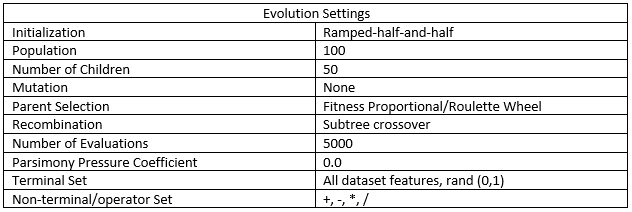
\includegraphics[width=0.8\columnwidth]{EASettings.png}
\caption{The settings that the EA used for the KMeansGP framework.}
\end{center}
\label{fig}
\end{figure}

The initialization of the population used ramped-half-and-half\cite{EibenAE2007}.  This method makes half the initial population random full binary parse trees.  The operators and terminals are randomly decided.  The other half of the population has their trees randomly generated too.  The different between second half and the first half is that the second half are not guaranteed to be full trees.

The initial population is of size 100.  Every generation will produce 50 children.  Each member and of the initial population and every child generated count as one evaluation.  An evaluation in this program is running the evolved tree with k-means one time.  The program is set to only allow 5000 evaluations.

Fitness is a calculated using using a combination of purity\cite{Manning2008} and Parsimony Pressure\cite{EibenAE2007}.  Purity is easy to implement and is fairly fast.  The Parsimony Pressure as described in Eiben text is used to reduce the fitness of large GP.  My fitness function look like Fitness = Purity(Solution) - C * Depth(Tree).  The C represents the Parsimony coefficient, which is configurable in the settings file.  The idea is that the larger the tree, the longer it takes to evaluate.  During the tuning of paramters, the author found that having a positive Parsimony coefficient harmed my solution purity.  So for the experiments, the Parsimony coefficient was set to 0.0.
\subsection{Timing/Purity Tests}
After the EA was done running, the test dataset was loaded into memory and the timing and purity tests were started.  Every 100 evaluations in the EA, the best individual was stored in for this testing segment.  This test goes though the the trees that were saved thoughout the run of the EA, and runs it 30 times versus the base k-means.  To make it fair the comparison between the evolved k-means and base k-means use the same initial starting points.  The average of the 30 runs is recorded for both the timing and purity.

\clearpage

\section{Experimental Results}
\subsection{Datasets}
For this project, the following datasets were taken for the UCI Machine Learning Repository: Iris, Wine, and Isolet\cite{Dua:2017}.  The Iris dataset has 150 points in it and each point consists of four features.  The Wine dataset consists of 178 points and each point consists of 13 features.  Finally, the Isolet dataset has 7797 points and each point has 617 attributes.

There is good reasoning why these particular datasets were chosen.  The first is that these datasets do not have any missing values.  Normalization would have been possible on many other datasets in the UCI Machine Learning Repository, but dealing with the error that can introduce was not something author wanted to introduce into the experiment.  Next, all three datasets use numerical types on the features.  This was done so that the C++ implementation did not have to involve using templates, which would have increased compilation time.  Also, using non-numerical types would have involved some sort normalization, which the author was not interested in investigating for this project.  The Iris and Wine datasets were chosen because they both have about the same number points in them, but the number of features they have are fairly different.  This difference in the number of features would allow the author to investigate if the number of features affects the result of the experiment.  The Isolet dataset was chosen because it has a large number points and features when compared to Iris and Wine.  Looking at how the code handled the large dataset was something that needed to be included to this project.  Something to make a note of is that for all of the datasets used for this experiment, 80 percent of the dataset was used for training and 20 percent was used for testing.  Isolet was already split up this way.  Iris and Wine had to be randomly split into training and testing datasets.
\subsection{Purity}
Purity was used as the way to check the validity of the results of clustering.  It appears that the evolved k-means outperformed the base k-means on both Iris and Wine.  The evolved k-means for the Isolet dataset did not perform that well versus the base k-means.  The author believes that evolved k-means for Isolet does not perform that well because it has such a large number of features.  It is possible that the initial population of the EA did not capture the most important features in the parse trees, possibly causing such poor results.
\begin{figure}[H]
\begin{center}
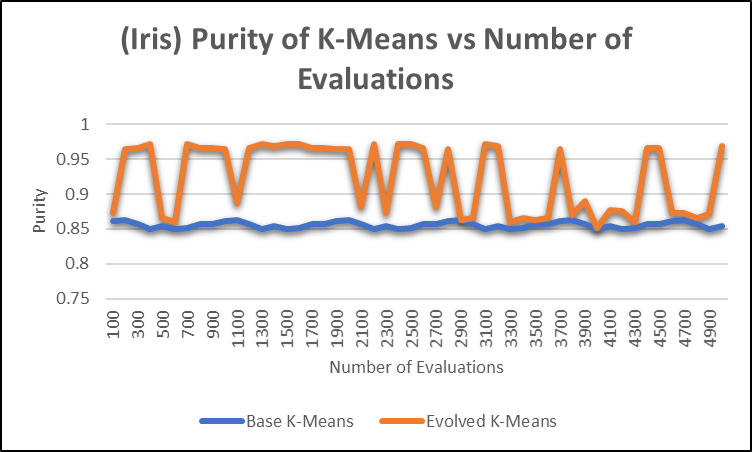
\includegraphics[width=0.7\columnwidth]{irispurity.png}
\caption{Purity of Iris test dataset.}
\end{center}
\label{fig}
\end{figure}
\subsection{Timing}
The timing of the evolved k-means versus the base k-means for each of the datasets was recorded for this experiment.  The goal of this project was to reduce the run time of k-means.  When looking at the timing results for both Iris and Wine, the evolved k-means is almost always slower than the base k-means clustering.  Now looking at the timing results on the Isolet dataset, the evolved k-means is about one second faster than the base k-means.  This result may look good initially, but the evolved k-means has on average a 0.4 lower purity compared to base k-means.
\begin{figure}[H]
\begin{center}
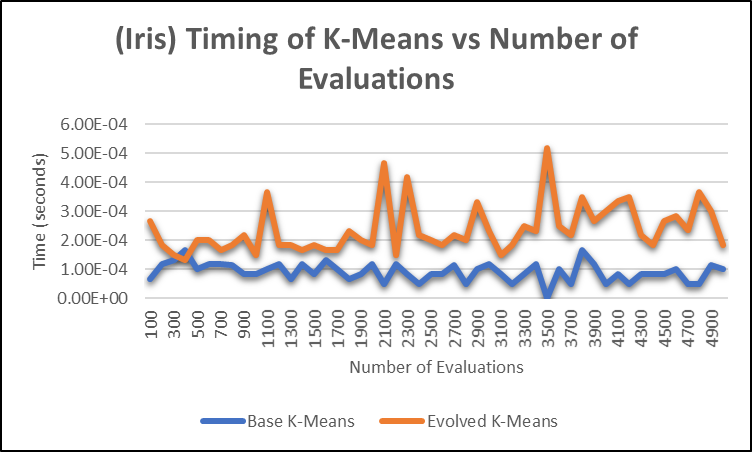
\includegraphics[width=0.7\columnwidth]{iristiming.png}
\caption{Timing of Iris test dataset.}
\end{center}
\label{fig}
\end{figure}

\subsection{Conclusions}
Looking at the goal for improved timing of k-means, the KMeansGP framework failed to produce the desired results.  An unintended result was how the evolved k-means for both Iris and Wine had a higher purity over almost all the evaluations.  This makes sense since the EA was evolving with the fitness being the purity.  The intention was to evolve on the purity so the solution produced by the featured reduce k-means would not lose accuracy in its solution.
\subsection{Future Work}
As almost any computer programmer will tell you, there are always things that you can improve with the code.  This project is no exception.  As suggested by Dr. Wunsch, applying this framework on a method with a higher time complexity than k-means would be more worthwhile.  The EA likely needs to have a built-in restart feature, as it appears the the population is getting stuck in a local maximum.  The framework needs to be able to do normalization on the data, this would open the ability to use datasets that have missing missing values and non-numeric features.  The functions in the code need to be more separated out than they are currently.  One of the biggest features that would be nice to have is a incorporating an EA that used less parameters.     
\clearpage

\onecolumn
\section{Acknowledgements}
I would like to thank my advisor, Dr. Daniel Tauritz, for his advice on getting started with this project and for teaching me much of the Genetic Programming techniques used in this paper.  My friend, Wyatt Kennedy deserves some recognition for asking me questions about my project so that I understand it better.  Thank you Dr. Donald Wunsch and Leonardo Enzo Brito Da Silva, for facilitating a classroom environment that inspired this project.  As requested by the citation policy of the UCI Machine Learning Repository, the author of this paper would like to thank the submitters of the datasets that were used in this project. 
\clearpage

\bibliographystyle{IEEEtran}
\bibliography{kmeansgp-bibliography} 

\onecolumn
\section{Appendix A}
All the code for this project can be found at the following link: \href{https://github.com/tuglight/KMeansGP}{https://github.com/tuglight/KMeansGP}\cite{KMeansGP}

\begin{figure}[H]
\begin{center}
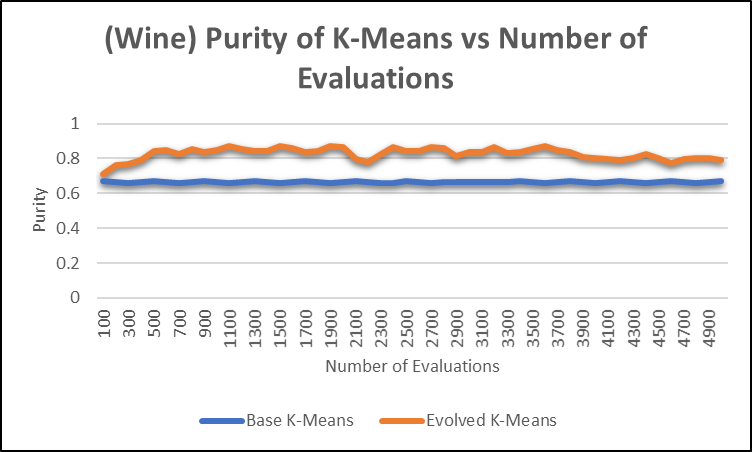
\includegraphics[width=0.7\columnwidth]{winepurity.png}
\caption{Purity of Wine test dataset.}
\end{center}
\label{fig}
\end{figure}

\begin{figure}[H]
\begin{center}
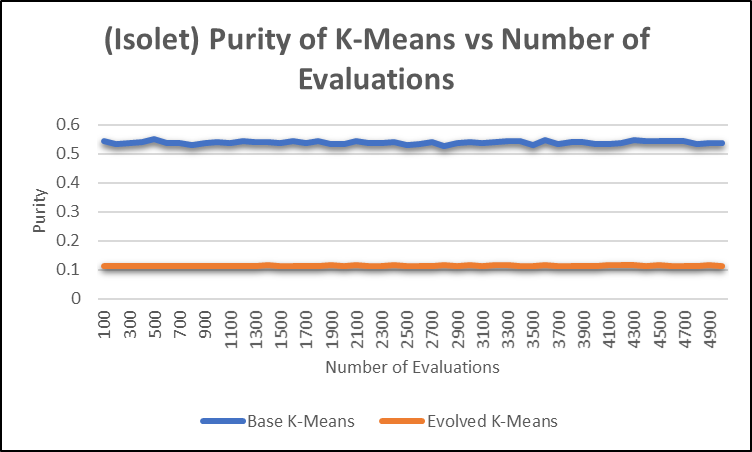
\includegraphics[width=0.7\columnwidth]{isoletpurity.png}
\caption{Purity of Isolet test dataset.}
\end{center}
\label{fig}
\end{figure}

\begin{figure}[H]
\begin{center}
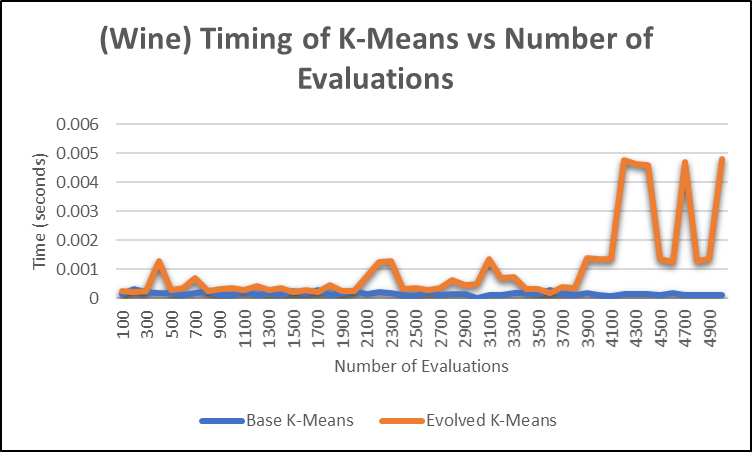
\includegraphics[width=0.7\columnwidth]{winetiming.png}
\caption{Timing of Wine test dataset.}
\end{center}
\label{fig}
\end{figure}

\begin{figure}[H]
\begin{center}
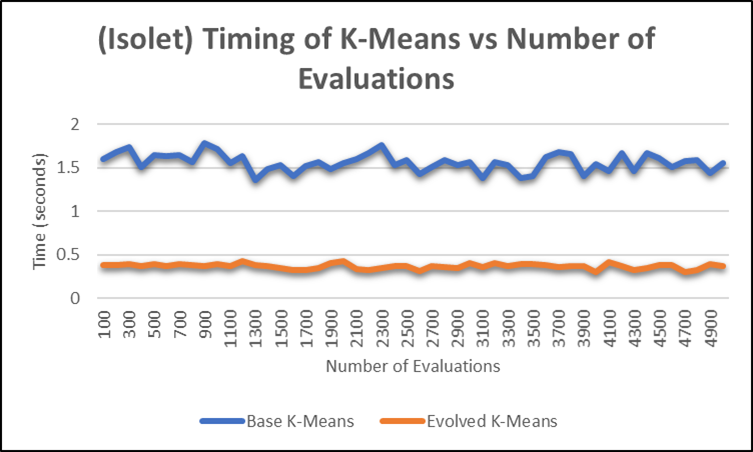
\includegraphics[width=0.7\columnwidth]{isolettiming.png}
\caption{Timing of Isolet test dataset.}
\end{center}
\label{fig}
\end{figure}

\end{document}